\documentclass[a4paper]{iacas}% insert '[draft]' option to show overfull boxes

\usepackage{hyperref}% embedding hyperlinks [must be loaded after dropping]
\usepackage{amsmath}
\usepackage{soul,color}
\usepackage{threeparttable}% tables with footnotes
\usepackage{dcolumn}% decimal-aligned tabular math columns
\newcolumntype{d}{D{.}{.}{-1}}
\usepackage{graphicx}
\usepackage{caption}
\usepackage{subfig}
\usepackage{multirow}

\title{Computational Fluid Dynamics Modeling of Cathodic Arc Jet in Stationary Atmospheric Pressure Gas}

\author{%
	Anton Ronis\thanks{Gradute Student. E-mail: ro@tx.technion.ac.il}
	\ and
	Igal Kronhaus\thanks{Assistant Professor. E-mail: kronhaus@technion.ac.il}\\
	{\normalsize\itshape
		Faculty of Aerospace Engineering, Technion, Haifa,
		3200003, Israel}
}

% define some commands to maintain consistency
\newcommand{\pkg}[1]{\texttt{#1}}
\newcommand{\cls}[1]{\textsf{#1}}
\newcommand{\file}[1]{\texttt{#1}}

\begin{document}
	
	\maketitle
	
	\begin{abstract}
		In this paper a computational fluid dynamic (CFD) model is developed. A comparison with measurement data is made using spatial distribution of flow parameters as well as a \emph{Taylor-Sedov} blast wave model analysis.
		The numerical solution is carried out using a modified \texttt{OpenFOAM} open source toolbox solver, based on the \texttt{icoFoam} solver. The \texttt{icoFoam} is a pressure based solver for transient incompressible flows which was modified to include an external force field acting on the flow.
		The flow properties -- pressure and velocity qualitatively analyzed in different periods of simulation time. The pressure front position and static values, caused by the jet expansion with respect to time, are sampled and compared to the results obtained from experiment and the \emph{Taylor-Sedov} blast model.
		The CFD jet model of the CAJ predicts well the observed phenomenons from experiments -- \emph{i.e.} forming of an initial cylindrical expansion zone at $1~\mu s$, steady conditions in the CAJ region after around $t = 100~\mu s$, and compatibility with the \emph{Taylor-Sedov} blast model pressure front position and velocity, with respect to time and distance, respectively. 
	\end{abstract}

\section{Introduction}
Active manipulation of flows is an important area of aeronautical research \cite{GADEL}. One prominent example is the use of flow manipulation to reduce drag by delaying and/or eliminating separation zones \cite{SIMPSON}. The literature provides several examples of flow-control devices including: bumps, vanes (vortex generators), synthetic jets, bleed/suction and plasma actuators.
In contrary to other actuators, plasma actuators can operate on the flow by three different mechanisms \cite{FLOWCTRL}: momentum, shock and chemical effects. Momentum effects induce near surface flow velocities. Shock effects induce very high local gas pressure and temperature which creates gradients in the background air. Chemical effects introduce new species, such as ions, electrons, excited particles into the flow field. The most studied plasma actuator configuration is the dielectric barrier discharge (DBD) which is capable of inducing $\sim10$ $m/s$ flows \cite{FLOWCTRL,KOK,WHALLEY,MOREAU}, too low to be effective at high subsonic regimes.

In a recent study \cite{KR}, cathodic arcs operating at atmospheric pressure environment were shown to produce fast jets of gas. This so called cathodic arc jet (CAJ) induces a local flow field velocities of $\ge$ 100 $m/s$ (see Fig. \ref{fig:CAJ}). The jet direction was also shown to be controlled by the application of an external magnetic field. Physical model of the CAJ was developed in a recent paper \cite{KRClose}, relating the cathode and background gas properties to the observed CAJ. The results suggest the possible use of a CAJ as a flow-control device for external subsonic flows\cite{KRFar}.

In this paper a computational fluid dynamic (CFD) model is developed. A comparison with measurement data is made using spatial distribution of flow parameters as well as a \emph{Taylor-Sedov} blast wave model analysis \cite{TAYLOR,SEDOV}.

\begin{figure}
	\centering
	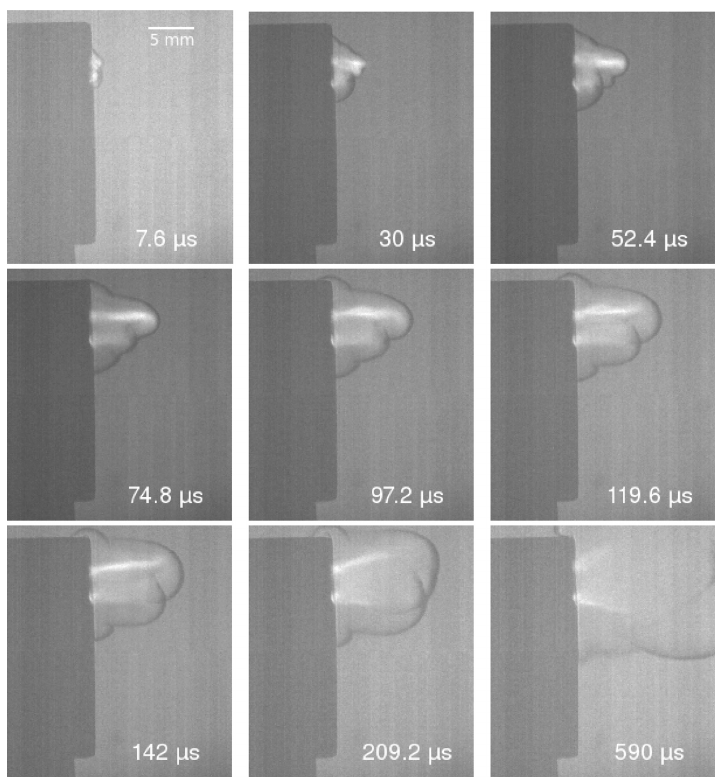
\includegraphics[width=0.6\textwidth]{CAJ_highres.png}
	\caption{Schlieren images of the cathodic arc jet in air. The luminous plasma shows white. The time is counted from the moment of ignition. Reproduced from \cite{KR}.}
	\label{fig:CAJ}
\end{figure}

%The numerical solution is carried out using a modified \texttt{OpenFOAM} \cite{OPENFOAM} open source toolbox solver, \texttt{forcedIcoFoam} \cite{NS}. The \texttt{forcedIcoFoam} is a pressure based solver for transient incompressible flows modified to include an external force field acting on the flow.
%
%The numerical approach is based on the assumption that the CAJ effect on the background gas can be simulated by an application of acceleration field which causes the gas to reach the velocities obtained in the \cite{KR}. Therefore the jet simulation corresponds to a hot gas expansion at a subsonic speed. Following measurement data \cite{KRClose}, the acceleration field was adjusted to yield a velocity of $500~ m/s$.
%
%The flow properties -- pressure and velocity qualitatively analyzed in different periods of simulation time. Sampling the pressure front position and static values, caused by the jet expansion with respect to time allows one to compare the results obtained from the simulation with \emph{Taylor-Sedov} blast model \cite{TAYLOR,SEDOV}  .
%The pressure front position and velocity obtained in a simulation are visualized in Fig. \ref{fig:model_position} and Fig. \ref{fig:model_velocity}, respectively. The results correspond well with the measured data in \cite{KR}.
%
%The CFD jet model of the CAJ predicts well the observed phenomenons from \cite{KR} -- \emph{i.e.} forming of an initial cylindrical expansion zone at $1~\mu s$, steady conditions in the jet area after around $t = 100~\mu s$, and compatibility with the \emph{Taylor-Sedov} blast model pressure front position and velocity, with respect to time and distance, respectively. Modeling the CAJ as a jet results in some deficiencies -- mainly the addition of mass to the background gas domain and the generation of vortices caused by the flow expansion at the inlet edge. These deficiencies are notable in the local jet domain and must be accounted for in the final CFD model of the CAJ. 
%
%

\section{Physical Model}\label{sec:physical_model}
The schlieren time sequence images in Fig. \ref{fig:CAJ} provide evidence for the following process in the formation of the CAJ:
\begin{enumerate}
	\item Plasma formation in a bounded region
	\item CAJ plume expansion towards the background gas
\end{enumerate}

In the first event a small yet energized volume of plasma particles is generated. A pressure boundary is formed with a radius size determined by the cathode parameters, discharge current and the background gas. The properties of this boundary radius are discussed in Subsection \ref{subs:boundary_radius}. 
Subsequently, the second event begins with an expansion of the initial energized volume pressure \cite{meunier1987experimental}. This expansion is followed by the formation of a jet caused by a momentum and energy transfer of the plasma particles to the gas. It is seen that after the initial boundary expansion certain \textit{steady-state} conditions are met in the jet plume region. The initial expansion and resultant gas jet are discussed in Subsection \ref{subs:CAJ_expansion}. 

\subsection{Plasma-Gas Boundary Radius}\label{subs:boundary_radius}

The force exerted on the plasma particles can be written as:

\begin{eqnarray}\label{eqn:plasma_force}
	F_i &= &\frac{M_i V_i f}{Z e} I_d
\end{eqnarray}

Where $M_i$ is the ion mass, $V_i$ is the ion velocity, $f$ is the ion current fraction, $Z$ is the charge state, $I_d$ is the current magnitude and $e$ is the electron charge.
Constraining an equilibrium of forces between the plasma and gas we can use Eq. \eqref{eqn:plasma_force} to express the area, $A$, for a given pressure, $p$, for which an equilibrium is achieved:

\begin{eqnarray}\label{}
	F_g & = & F_i \\\label{eqn:rel_equiv_force}
	p A & = & \frac{M_i V_i f}{Z e} I_d\\
	A & = & \frac{M_i V_i f}{Z e} \frac{1}{p} I_d
\end{eqnarray}

Where $F_g$ and $F_i$ are the background gas pressure force and the ion momentum transfer force, respectively. Assuming hemi-spherical distribution of the gas pressure force on the plasma, i.e $A = 2\pi r^2$, the following expression is obtained for the radius, $r$:

\begin{eqnarray}
\label{eqn:rad_equiv_force}
	r & = & \mathcal{C}\sqrt{I_d}
\end{eqnarray}


Where $\mathcal{C} = \sqrt{\frac{1}{2\pi}\frac{M_i V_i f}{Z e}\frac{1}{p}}$ is a constant defined by the cathode and experimental parameters. This allows us to relate the boundary radius $r$ to the discharge current, $I_d$, thus resulting in a simplified relation between the two, for a given set of cathode parameters. Results for the given parameters in the experiments \cite{KR,KRClose} are shown in Table~\ref{t:radii}.

\begin{table}[hbt]
	\begin{center}
		\begin{threeparttable}
			\caption{Calculated CAJ boundary radius}
			\label{t:radii}
			\begin{tabular}{l|c|c}
				\multirow{2}{*}{Parameter} & Case 1 & Case 2\\ 
				& $I_d = 230~\mathrm{A}$ & $I_d = 40~\mathrm{A}$\\\hline
				$p$ & $101 \times 10^3~\mathrm{Pa} $ & $101 \times 10^3~\mathrm{Pa} $ \\
				$T$	& $850~\mathrm{K}$ & $850~\mathrm{K}$ \\
				$\gamma$ & $1.365$ & $1.365$ \\ 
				$\mathrm{M}$	& $0.856$ & $0.856$ \\
				$M_i$  	& $1.055 \times 10^{-25}~\mathrm{kg} $ & $1.055 \times 10^{-25}~\mathrm{kg} $  \\
				$V_i$ 	& $12.5 \times 10^3~\mathrm{m/s} $ & $12.5 \times 10^3~\mathrm{m/s} $  \\
				$f$ 	& $0.08 $ & $0.08 $ \\
				$Z$	& $1.8 $ & $1.8 $ \\
				$\mathrm{M}$	& $0.856$ & $0.856$ \\
				$r$ 	& 0.35~mm & 0.14~mm
			\end{tabular}
		\end{threeparttable}
	\end{center}
\end{table} 

\subsection{CAJ Plume Expansion Region}\label{subs:CAJ_expansion}

The evolution of the initial pressure wavev due to the formation of plasma can be modeled using a \emph{Taylor-Sedov} blast wave model \cite{TAYLOR,SEDOV}: 

\begin{eqnarray}\label{eqn:taylor_sedov}
r^5 t^{-2} &=& \mathrm{constant}
\end{eqnarray}

The pressure wave initially starts with a sonic velocity of $\approx 500~\mathrm{m/s}$ at the plasma boundary \cite{KRClose}, and quickly decays to $\approx 50~\mathrm{m/s}$ \cite{KR,KRFar} at $\approx 10~\mathrm{mm}$ as visualized in Fig. \ref{fig:CAJ}.

Following the pressure wave expansion is the formation of the CAJ at the plasma-gas boundary. The CAJ is assumed to follow the initial pressure wave expansion velocities close to the boundary, and then decrease in velocity with the increase of distance from the boundary. The steady-state results, summarized in Table~\ref{t:radii}, show that an equilibrium is achieved for distances of less than 1~mm. We can therefore assume that for $> 1~\mathrm{mm}$ a decay in the plasma density occurs.

Following the CAJ model developed in \cite{KRClose} we assume that the CAJ is formed mainly doe to momentum transfer from ions to the gas. In steady state conditions at the plasma-gas boundary, with constant current, $I_d$, we can express the exerted force on the gas with respect to velocity as:

\begin{eqnarray}\label{eqn:force_mass_flux}
	F_g &=& \dot{m} V_g
\end{eqnarray}

Substituting the mass flux $\dot{m}$ for $\rho V_g A_{o}$ -- where $A_{o}$ represents a circular cross section through which the jet flows and $\rho$ is the fluid density, yields:

\begin{eqnarray}\label{eqn:force_density}
F_g &=& \rho V^2_g A_{o}
\end{eqnarray}

However, we know that the boundary radius defined by an equivalence between the pressure force and the ion force. Comparing the former with 
Eq. \eqref{eqn:force_density} thus yields:

\begin{eqnarray}\label{eqn:force_gas_equal}
p A &=& \rho V^2_g A_{o}
\end{eqnarray}

Substituting the areas $A$ and $A_o$ with the relevant expressions involving the boundary radius, $r$ results in: 

\begin{eqnarray}\label{eqn:force_gas_ratio}
p \cdot 2\pi r^2 &=& \rho V^2_g \cdot 2\pi r^2 \\
\frac{p}{\rho} &=& \frac{V^2_g}{2}
\end{eqnarray}

Using the state equation for an ideal gas, $pV = NRT$, we get:

\begin{eqnarray}\label{eqn:force_gas_temperature}
	T &=& \frac{V^2_g}{R}
\end{eqnarray}

Where $T$ is the temperature and $R$ is the specific gas constant. Eq. \eqref{eqn:force_gas_temperature} relates the gas temperature to the jet velocity. Substituting $R = 287~J\cdot kg^{-1} K^{-1}$ and $V_g = 500~m/s$ results in a temperature values of around 850 K. From here we can express the Mach number at the boundary, as:

\begin{eqnarray}
	\mathrm{M} &=& \frac{V_g}{a} \\
	 &=& \frac{\sqrt{RT}}{\sqrt{\gamma R T}}\\\label{eqn:mach}
	 &=& \sqrt{\frac{1}{\gamma}}
\end{eqnarray}

For most cases, the heat capacity ratio $\gamma \geq 1$. %Specifically for ideal air at $1000^o~C$ $\gamma = 1.365$ -- We can therefore conclude that the boundary Mach is $\mathrm{M} = 0.856$. 
Values of Mach and Temperature are summarized in Table~\ref{t:radii} for dry air.

\section{Numerical Model}

The CFD numerical approach is derived from the assumption that the CAJ is formed predominantly due to momentum transfer caused by collisions between ion and background gas particles and therefore can be simulated by an application of acceleration field which causes the gas to reach the velocities measured in \cite{KR}. This corresponds to adding a body force acceleration to the Navier-Stokes momentum equations:

\begin{eqnarray}
\label{eqn:NS-Force}
\frac{\partial \boldsymbol{u}}{\partial t} + (\boldsymbol{u} \cdot \nabla)\boldsymbol{u} &=& -\frac{1}{\rho}\nabla p + \frac{\mu}{\rho} \nabla^2 \boldsymbol{u} + \boldsymbol{F_b}
\end{eqnarray}

Where $\boldsymbol{u}$ is the flow field velocity and $\boldsymbol{F_b}$ represents the acceleration field.

The numerical solution is carried out using a modified \texttt{OpenFOAM} \cite{OPENFOAM} open source toolbox solver, based on the \texttt{icoFoam} solver. The \texttt{icoFoam} is a pressure based solver for transient incompressible flows which was modified to include an external force field acting on the flow. An incompressible solver was used due to its simplicity and fast calculation time. It is therefore important to note that compressibility effects are not taken into account. The use of an incompressible solver can be justified by the fact that $\mathrm{M} < 1$ at boundary, as described in Section \ref{sec:physical_model}.

The numerical domain consists of 200 $\times$ 300\footnote{Grid dimensions were obtained by conducting grid size sensitivity runs, analyzing the CAJ profile} grid points representing a 15 mm $\times$ 30 mm dimensioned physical domain. The grid density is adjusted at the wall region to yield a maximal cell height of 0.1~mm. 

We simulate the plasma-gas interaction by assuming a constant acceleration field just beneath the CAJ expansion plume region. The field properties are calculated to correspond with the plasma-gas boundary given in Eq. \eqref{eqn:rad_equiv_force}. For the observed parameters representing the experiment \cite{KR} of Fig.~\ref{fig:CAJ}, the field was placed at $ y < 0.5~ \mathrm{mm} $ at a width of $r = 1~\mathrm{mm}$, centered around $x=0~\mathrm{mm}$. These values correspond to a discharge current of 230 A (Case 1 in Table~\ref{t:radii}).
Following the measurement data in \cite{KRClose}, the acceleration field is adjusted to yield a velocity of $500~ m/s$. It is assumed that the discharge current affects only the initial CAJ expansion location which in turn is defined by the background gas properties - Eq. \eqref{eqn:rad_equiv_force}. The gas is assumed to be stationary, with atmospheric pressure at room temperature.

\section{Results \& Discussion}

The simulation is executed at a modified time step constraining the Courant number $\mathcal{C} \leq 0.1$, for a total simulation time of $t = 500~\mu s$. The solution region of interest corresponds with the CAJ plume expansion region ($ y > 1 \mathrm{mm} $). The velocity and pressure field spatial distributions, obtained at $ t = 500~\mu s $, are illustrated in Fig. \ref{fig:velocity_field} and Fig. \ref{fig:pressure_field}, respectively. The acceleration field results in the formation of a time evolving axisymmetric jet that reaches pseudo-steady-state conditions by $t = 500~\mu s$.
The pressure front position and velocity obtained in a simulation are visualized in Fig. \ref{fig:model_position} and Fig. \ref{fig:model_velocity}, respectively. There's a very good correspondence between the Taylor-Sedov \cite{TAYLOR,SEDOV} Blast model and the pressure/velocity front velocities obtained in the simulation. The measurement results of \cite{KR} show good agreement with the CFD results.

The pressure front velocity and the CAJ velocity profile evolution are depicted in Fig. \ref{fig:model_caj_velocity}. We observe that the velocity profile developed in the CAJ  follows the pressure's front velocity moreover, the former one is larger in magnitude. The two velocities converge as the CAJ reaches $> 18~\mathrm{mm}$. 

The CAJ axial velocity gradient with respect to axial distance from the cathode is shown in Fig. \ref{fig:model_caj_acceleration}, for several times. For each instantaneous moment, we can observe a sharp decrease of the gradient magnitude at a certain distance from the cathode spot. We note that the gradient values converge to a distance of about 6~mm (dotted vertical line). It is interesting to note the correspondence of this location with the bright spot of the CAJ observed in \cite{KR}.

\begin{figure}
	\centering
	
	\subfloat[Velocity]{
		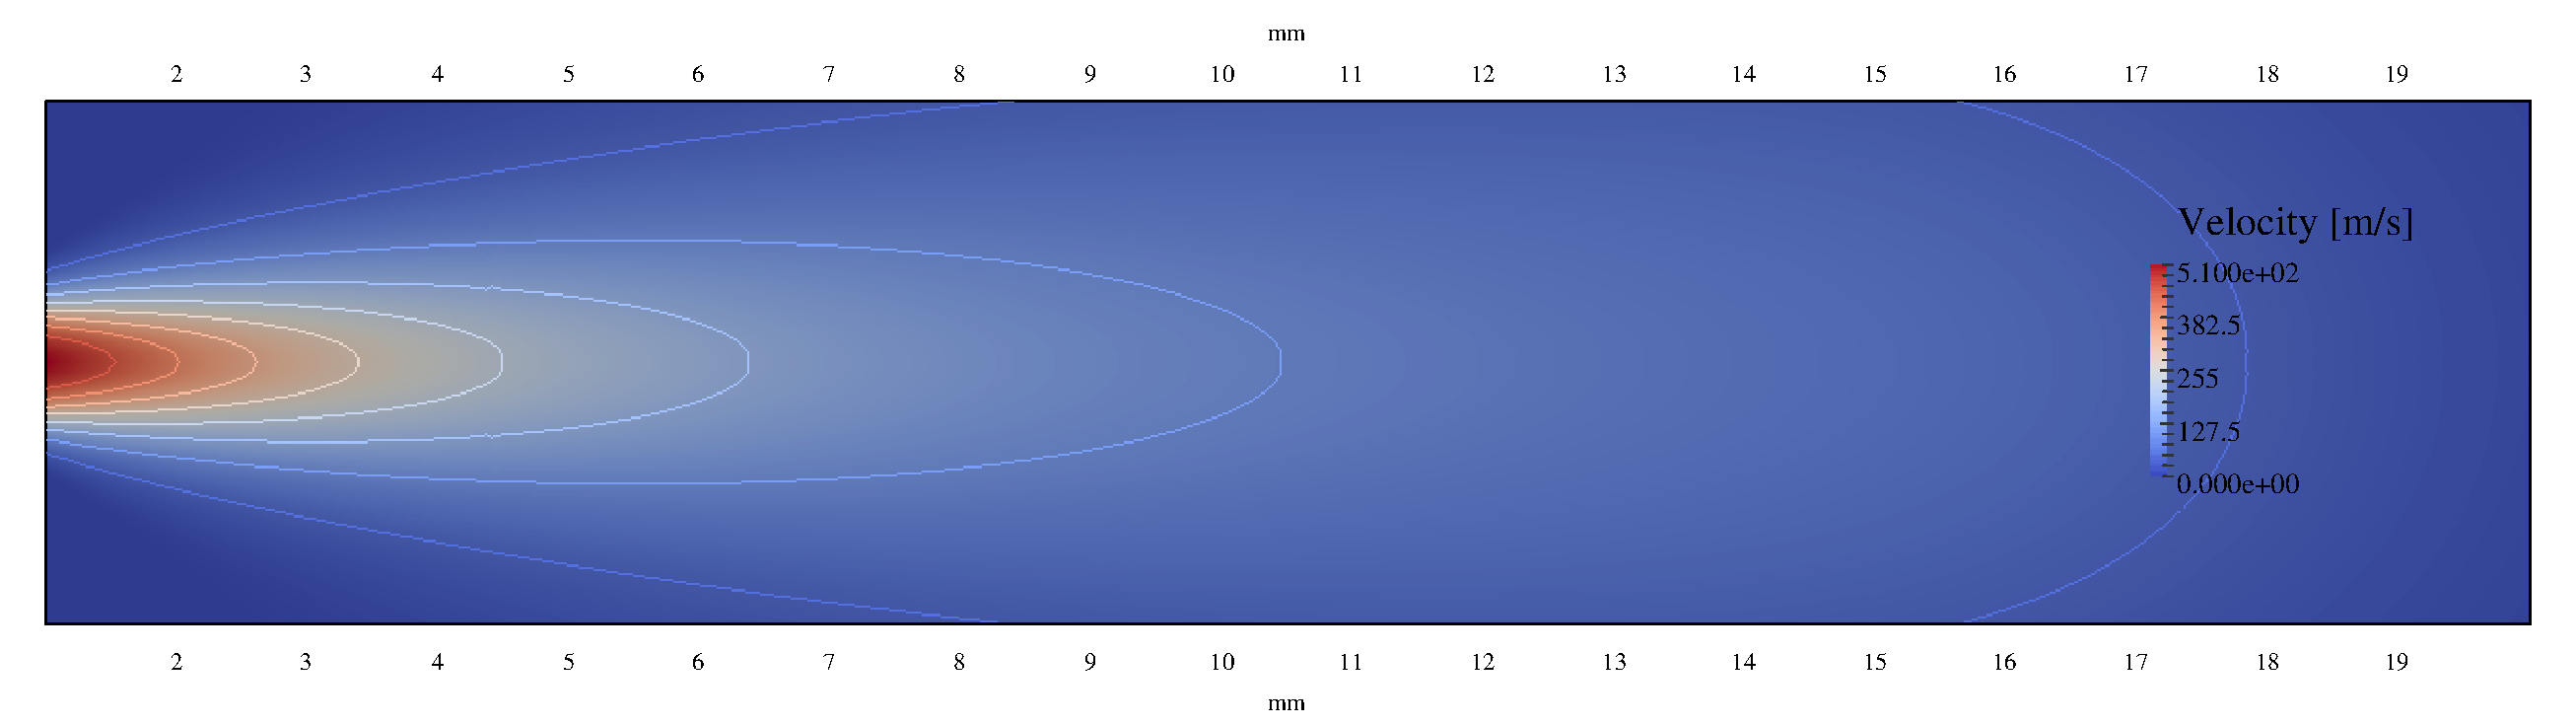
\includegraphics[width=0.9\textwidth]{velocityField}
		\label{fig:velocity_field}
	}
	
	\subfloat[Pressure]{
		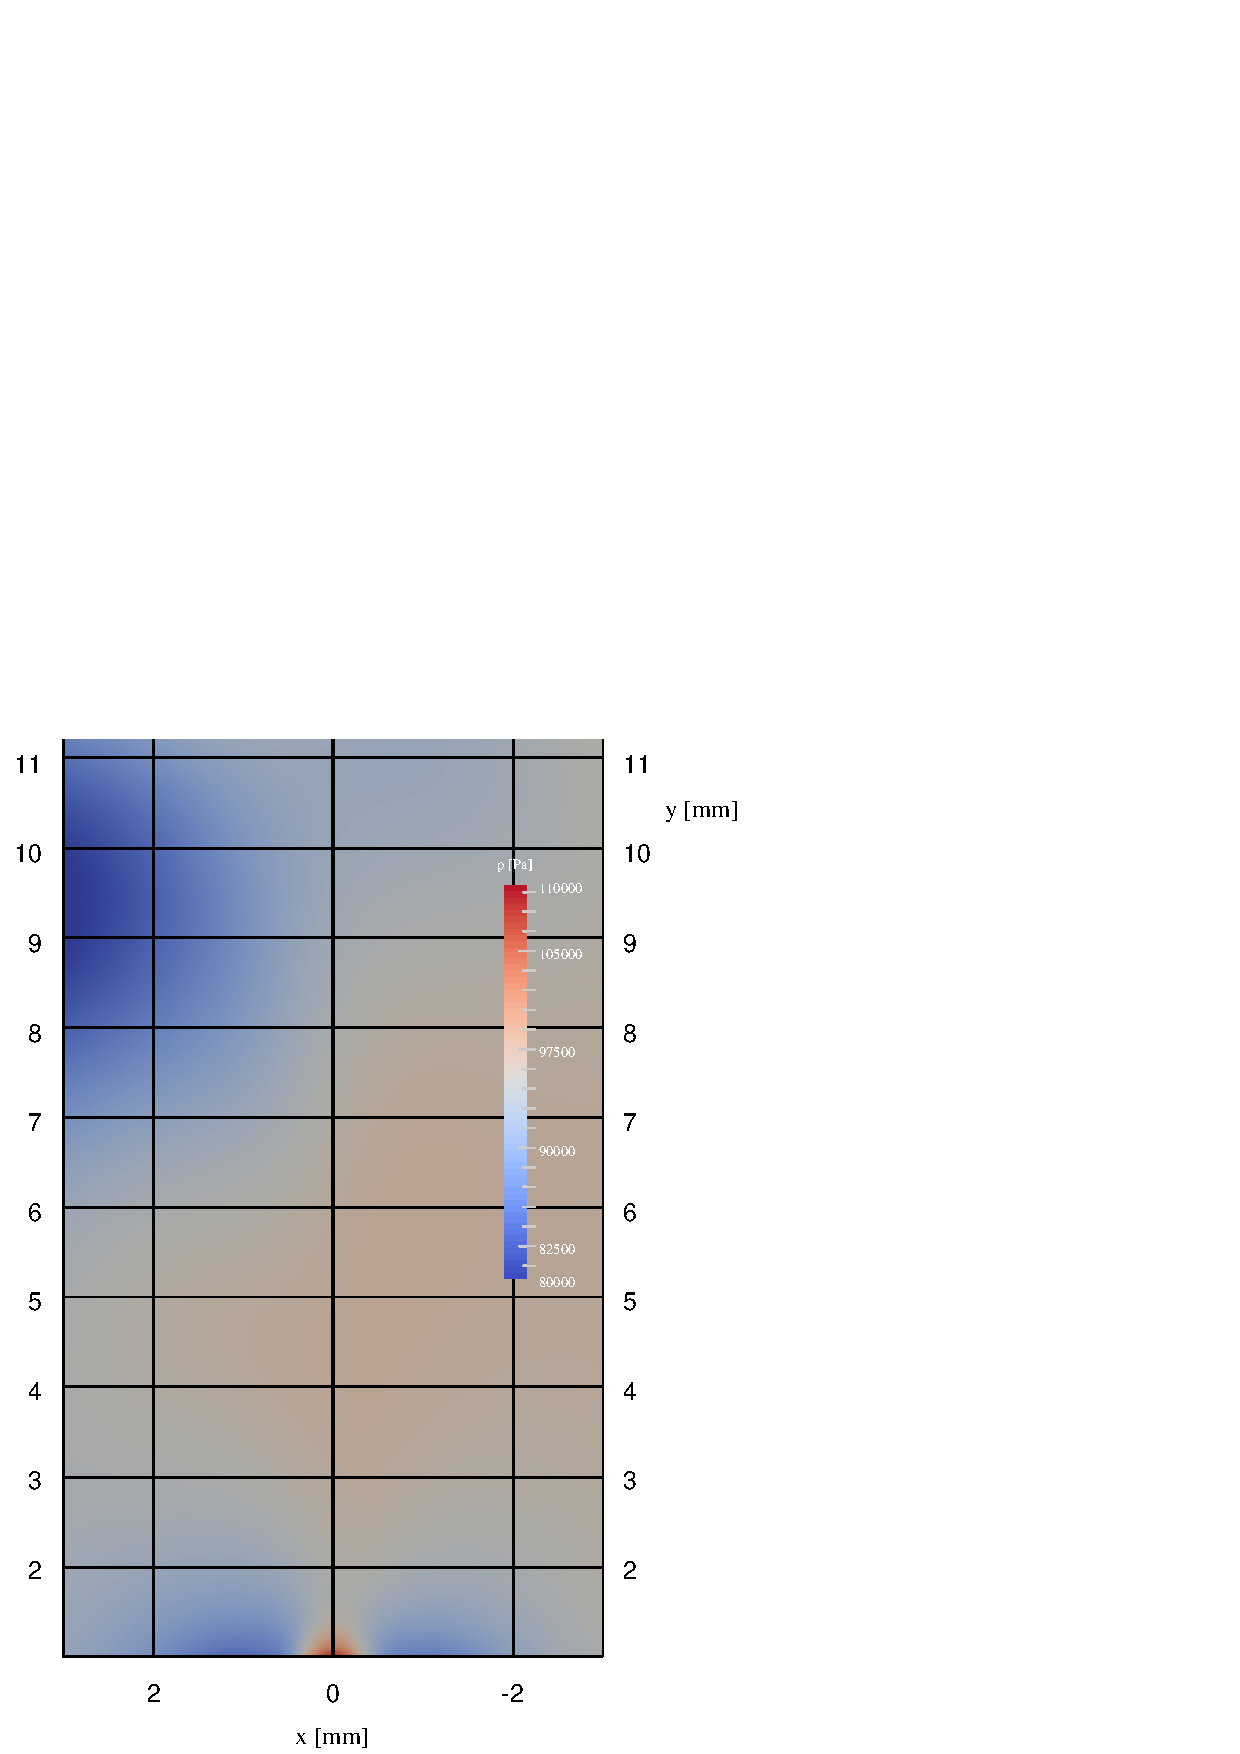
\includegraphics[width=0.9\textwidth]{pressureField}
		\label{fig:pressure_field}
	}
	\caption{(a) Velocity field, $ t = 500~\mu s $; (b) Pressure field, $ t = 500~\mu s $}
\end{figure}

\begin{figure}
	\centering
	\subfloat[Position]{
		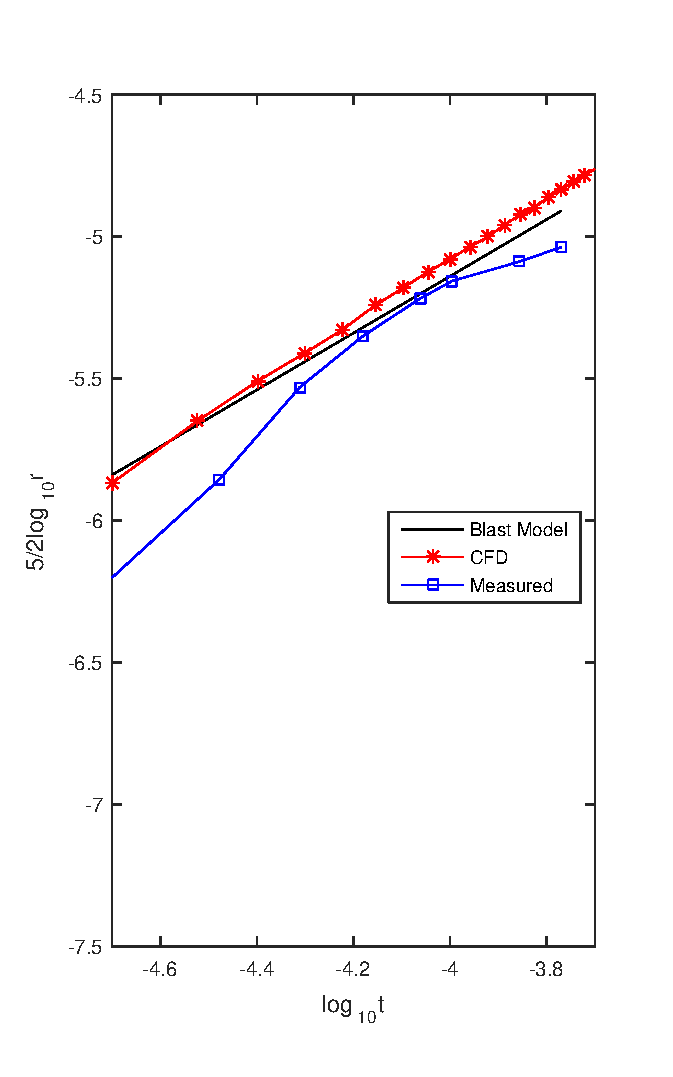
\includegraphics[width=0.28\textwidth]{ModelJetPosition.eps}
		\label{fig:model_position}
	}
	\subfloat[Velocity vs. Position]{
		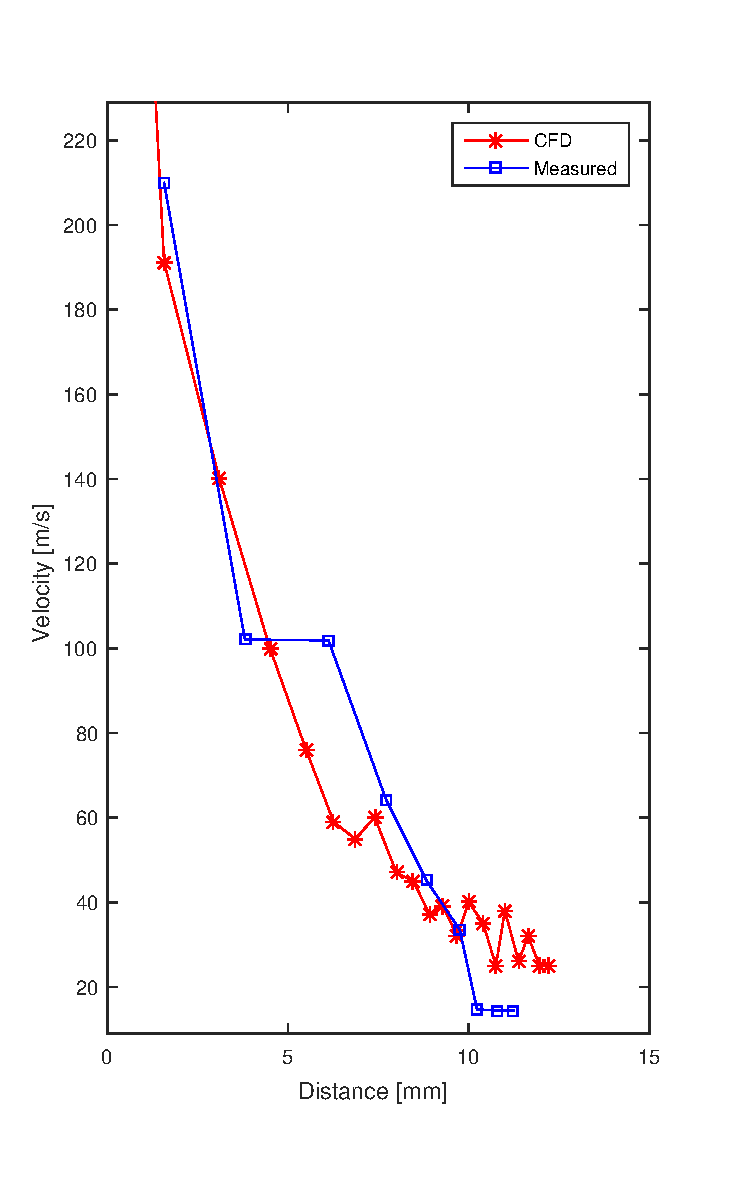
\includegraphics[width=0.28\textwidth]{ModelJetVelocity.eps}
		\label{fig:model_velocity}
	}
	\caption{(a) Time evolution of gas pressure front position (squares - experiment, stars - CFD) together with a linear fit of the blast wave model (black line); (b) the gas pressure front velocity versus position, measured in the direction of the plasma jet (squares) together with the computed CFD velocity of the front (stars). Experiment data reproduced from \cite{KR}.}
	\label{fig:model_blast}
\end{figure}

\begin{figure}
	\centering
	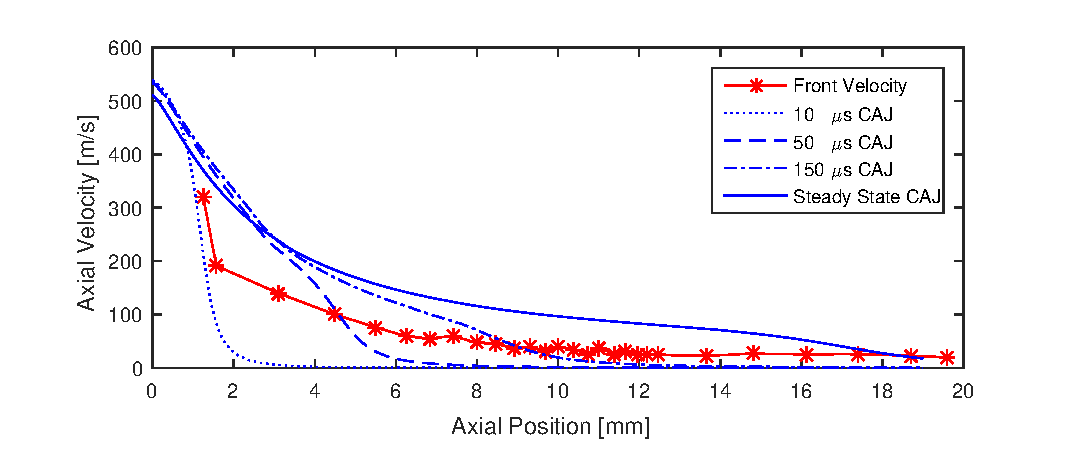
\includegraphics[width=0.6\textwidth]{Vel_Times.eps}
	\caption{Front expansion rate (red squares); Time evolution of the CAJ axial velocity versus axial position for sample times of $10~\mu s$, $50~\mu s$, $100~\mu s$, $150~\mu s$ and Steady state conditions (blue line).}
	\label{fig:model_caj_velocity}
\end{figure}

\begin{figure}
	\centering
	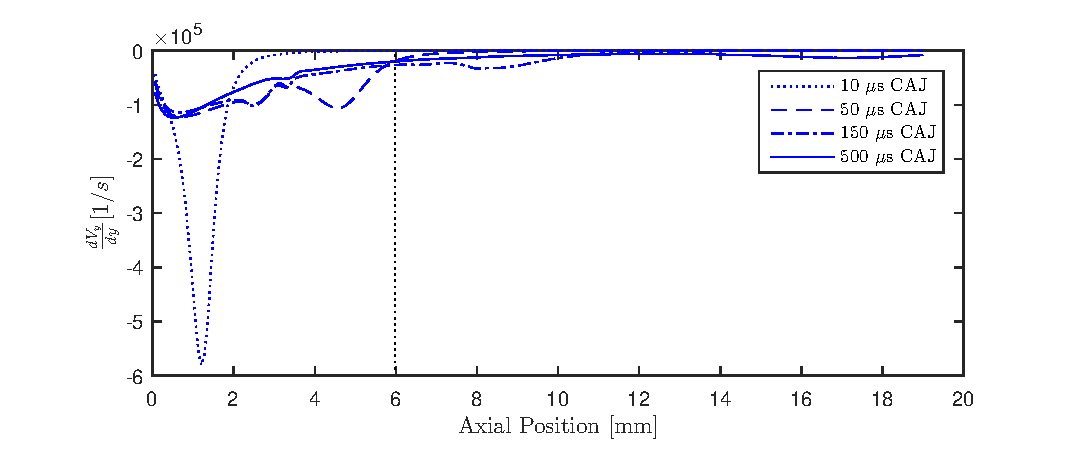
\includegraphics[width=0.6\textwidth]{CAJAcceleration.eps}
	\caption{Time evolution of the CAJ axial velocity gradient with respect to the axial distance from the cathode, for sample times of $10~\mu s$, $50~\mu s$, $100~\mu s$, $150~\mu s$ and Steady state conditions (blue line); $-2\cdot 10^4~1/s$ horizontal boundary line (black dash); the vertical line (black dotted) indicates the position where the gradient cross at different times. }
	\label{fig:model_caj_acceleration}
\end{figure}

\section{Conclusions}
A CFD model of the cathodic arc jet was developed and its results were compared with measurement data, as well with a \emph{Taylor-Sedov} blast wave model.
An \texttt{OpenFOAM} incompressible solver was modified to include a region of external force field, simulating the acceleration of the background gas due to the plasma ions momentum transfer.
The flow properties -- pressure and velocity were qualitatively analyzed in different periods of simulation time. The CFD results show a good corresponds with measurements found in the literature \cite{KR,KRClose,KRFar}. The pressure front position and static values, caused by the jet expansion with respect to time, show that the steady-state velocity is higher than the transient front velocity with $> 100~m/s$ at a distance of $10~\mathrm{mm}$.
The CFD jet model of the CAJ predicts well the observed phenomenons from experiments -- \emph{i.e.} forming of an initial hemispherical expansion zone at transient and steady conditions in the CAJ. Further studies are to be conducted analyzing the effects of a cross-flow on the CAJ based on the suggested implementation of the model.

\clearpage
\bibliography{bibtex_database}
\bibliographystyle{iacas}
\end{document}


%%% Local Variables:
%%% mode: latex
%%% TeX-master: t
%%% End:
